
%%%%%%%%%%%%%%%%%%%%%%% file typeinst.tex %%%%%%%%%%%%%%%%%%%%%%%%%
%
% This is the LaTeX source for the instructions to authors using
% the LaTeX document class 'llncs.cls' for contributions to
% the Lecture Notes in Computer Sciences series.
% http://www.springer.com/lncs       Springer Heidelberg 2006/05/04
%
% It may be used as a template for your own input - copy it
% to a new file with a new name and use it as the basis
% for your article.
%
% NB: the document class 'llncs' has its own and detailed documentation, see
% ftp://ftp.springer.de/data/pubftp/pub/tex/latex/llncs/latex2e/llncsdoc.pdf
%
%%%%%%%%%%%%%%%%%%%%%%%%%%%%%%%%%%%%%%%%%%%%%%%%%%%%%%%%%%%%%%%%%%%


\documentclass[runningheads,a4paper]{llncs}

\usepackage{amssymb}
\usepackage{amsmath}
\setcounter{tocdepth}{3}
\usepackage{graphicx}
\usepackage{verbatim}
\usepackage{subcaption}
\captionsetup{compatibility=false}

\usepackage{url}
\urldef{\mailsa}\path|{alfred.hofmann, ursula.barth, ingrid.haas, frank.holzwarth,|
\urldef{\mailsb}\path|anna.kramer, leonie.kunz, christine.reiss, nicole.sator,|
\urldef{\mailsc}\path|erika.siebert-cole, peter.strasser, lncs}@springer.com|    
\newcommand{\keywords}[1]{\par\addvspace\baselineskip
\noindent\keywordname\enspace\ignorespaces#1}

\DeclareMathOperator*{\argmin}{arg\,min}

\begin{document}

\mainmatter  % start of an individual contribution

% first the title is needed
\title{What makes a query temporally sensitive?}

% a short form should be given in case it is too long for the running head
\titlerunning{What makes a query temporally sensitive?}

% the name(s) of the author(s) follow(s) next
%
% NB: Chinese authors should write their first names(s) in front of
% their surnames. This ensures that the names appear correctly in
% the running heads and the author index.
%

%\author{Alfred Hofmann
%\and Ursula Barth\and Ingrid Haas\and Frank Holzwarth\and\\
%Anna Kramer\and Leonie Kunz\and Christine Rei\ss\and\\
%Nicole Sator\and Erika Siebert-Cole\and Peter Stra\ss er}
%
\authorrunning{}
% (feature abused for this document to repeat the title also on left hand pages)

% the affiliations are given next; don't give your e-mail address
% unless you accept that it will be published
%\institute{Springer-Verlag, Computer Science Editorial,\\
%Tiergartenstr. 17, 69121 Heidelberg, Germany\\
%\mailsa\\
%\mailsb\\
%\mailsc\\
%\url{http://www.springer.com/lncs}}

%
% NB: a more complex sample for affiliations and the mapping to the
% corresponding authors can be found in the file "llncs.dem"
% (search for the string "\mainmatter" where a contribution starts).
% "llncs.dem" accompanies the document class "llncs.cls".
%

\toctitle{Lecture Notes in Computer Science}
\tocauthor{Authors' Instructions}
\maketitle


\begin{abstract}
\keywords{We would like to encourage you to list your keywords within
the abstract section}
\end{abstract}


\section{Introduction}

A basic intuition in temporal information retrieval research is that time should be modeled explicitly when scoring and ranking documents with respect to users' queries. Time-related criteria such as recency, currency, and freshness have long been recognized as factors in studies of relevance\cite{Barry1998}. Based on these criteria, information retrieval researchers have explored a variety of temporal retrieval models \cite{Li2003,Efron2011,Dakka2012} that explicitly incorporate time into the document ranking. These researchers refer to general classes of ``temporal queries'' or ``temporal information needs.''  Models have been proposed and evaluated for ``recency queries'' \cite{Li2003,Efron2011}, ``time-sensitive queries'' \cite{Dakka2012}, ``implicitly temporal queries'' \cite{Metzler2009}, and ``temporally biased queries'' \cite{Jones2007}. For evaluation, these studies rely on manual classifications of topics into temporal categories.

In this paper, we take a deeper look into these manually classified topics to develop a clearer understanding of \emph{what makes a query temporally sensitive}? While many researchers have relied on these manually classified topics, the methods used for classification are not clearly explained.  Researchers often refer to vague concepts of ``newsworthiness'' or a ``bona fide temporal dimension'' of topics with out clear explication of the criteria or processes used in classification. As such, using these manually classified topics for evaluation is of limited value, since we cannot be clear about the process that is being modeled. The study presented in this paper is a necessary step in temporal information retrieval research.

To address our question, we analyze over 600 topics from the Text Retrieval Conference (TREC) previously used in the experimental evaluation of temporal retrieval models. We employ qualitative techniques to identify characteristics of topics that might affect manual assessment of ``temporality.'' The resulting coded topics are used in a set of regression analyses to determine the specific relationships between these characteristics and manually assigned categories. Finally, we use the coded topics to predict when temporally-sensitive retrieval models might be effective.

This paper is structured as follows....

\section{What is a TREC topic?}
The test collections developed for TREC generally consist of a collection of documents, a set of topics, and a set of relevance judgments. Although the method of creation has changed over time, TREC topics are generally intended to mimic real users' information needs. Topics are contained in a set of structured text files associated with the test collection and generally consist of a title and description. Some collections include more detailed narratives, while others may have only a short title or query string without a detailed description of the information need.

The concept of  an \emph{information need} has been extensively discussed in the information science literature and is widely used in the information retrieval community. Here we define an \emph{information need} as the unobservable motivation behind individual users' information seeking. Information needs reflect the individual user's current state of mind and context, including social and cultural environments. While information needs themselves are not observable, user's information seeking behaviors -- including queries and document relevance judgements -- are incomplete but observable evidence of the underlying need. 

We believe that this definition captures the spirit of the concept of \emph{information need} as commonly used in information retrieval research, particularly in the case of ``topics'' in TREC.

\subsection{Time and relevance}

There are numerous notions of temporality in information retrieval research, each of which requires different methodologies for analysis. In this study, we are primarily concerned with what we term as \emph{temporal relevance}. We define this as the condition where information needs are satisfied by documents published at particular points in time. We distinguish this from \emph{temporal topicality} which refers to information needs that are satisfied by documents about certain periods in time. Of course, an information need may combine the two conditions (e.g., find documents about the Wars of the Roses published in the 1800s). Examples of studies concerned with temporal topicality include \cite{Berberich2010,Kanhabua2011}.

There are, of course, other notions of temporality in information retrieval research. For example, \emph{temporal relevance dynamics} is concerned with how the relevance of a document changes with respect to an information need over time \cite{Mizzaro1997}; \emph{temporal query dynamics} is concerned with the study of how queries are issued over time \cite{Shokouhi2011,Vlachos2005,Parikh2008,Lavrenko2000}; and \emph{temporal content dynamics} is concerned with the effects of content changes over time \cite{Kulkarni2011}.

In the next section we review examples of studies focused on  \emph{temporal relevance}.

\subsection{Time-sensitive queries}
Temporal relevance is concerned with conditions where documents published at particular points in time are considered more or less relevant than those published at other times. This condition is studied independent of or in conjunction with traditional topical retrieval models. In this section, we review how researchers in this area operationalize the concept of time and define the temporal characteristics of queries in their studies. 

Li and Croft's study of ``recency queries''  \cite{Li2003} was the first in this line of research. They hypothesize that some queries are ``recency queries'' where the most recently published documents are more likely to be relevant. They analyze queries associated with TREC topics 301-400 from TREC disks 4 and 5. Through the direct analysis of the temporal distribution of judged relevant documents, they classify 36 of the queries as recency queries because they have ``more relevant documents in the recent past.''

Jones and Diaz \cite{Jones2007} study the temporal characteristics of queries with the goal of query classification through the analysis of three TREC news collections and a web search engine log. They use the Associated Press (1988, 1989) and Wall Street Journal (1990-1992) collections from TREC disks 1 and 2 as well as the AQUAINT corpus with the 2003 Novelty track topics. They define three classes of queries based on the temporal distribution of pseudo-relevant documents: temporally ambiguous (requesting multiple events),  temporally unambiguous (requesting a single event), and atemporal (having no preference). They employed annotators to  manually classify 100 TREC queries based only on the topic title, description, and narrative. Specific criteria for classification are not given. For the AP and WSJ collections, they found that all of the queries were either atemporal or temporally ambiguous. As a result, they incorporated the 2003 Novelty track because it includes topics classified as ``event'' or ``opinion,'' which the authors found to correspond to the ``temporally unambiguous'' and ``atemporal'' categories. 

Expanding on the work of Li and Croft, Dakka et al \cite{Dakka2012} investigate a broader class of queries which they refer to as ``time-sensitive.'' They hypothesize that there are queries for which more relevant documents are found at specific points in time, not just recently. They evaluate their models using a subset of TREC disks 4 and 5, manually identifying a subset of topics 301-450 that they consider to be ``time-sensitive.'' To do so, they manually examine the title, description and narrative of each topic and identify queries associated with specific news events. If the topic information is insufficient to make a decision, they analyze the distribution of relevant documents. This resulted in a collection of 86 temporally sensitive queries. The document collection used for evaluation was restricted to the Financial Times (1991-1994) and Los Angeles Times (1989-1990) sub-collections.

Also expanding on the work of Li and Croft, Efron and Golovchinsky \cite{Efron2011} investigate additional models for recency queries. They use subsets of several TREC ad-hoc collections including the Associated Press documents from disks 1 and 2 with topics 101-200; Los Angeles Times and Financial Times documents from disks 4 and 5 with topics 301-450. They classify queries as ``recency'' or ``non-recency'' based on an analysis of the distribution of relevant documents. If at least 2/3 of relevant documents appear after the median document time, the query is considered a candidate for recency. Candidate queries are then manually reviewed to determine if they have a ``bona fide'' temporal dimension. However, the criteria for manual review were not specified.  The authors developed a second test collection using the Twitter API. Two users of an experimental Twitter search engine were asked to create two types of queries: recency and non-temporal. Recency queries were defined as ``queries where relevant tweets were necessarily written recently.''  Relevance judgments were collected via AMT. 

Finally, Peetz, Meij, and Rijke \cite{Peetz2013} investigate the effect of temporal bursts in estimating query models. Building on the above studies, they evaluate their models using the above test collections. In addition, they introduce the Blogs06 collection. As previously, the authors construct a subset of ``temporal'' queries through manual evaluation of topic descriptions and relevant document distributions. No specific criteria for classification are given.

\subsection{What makes a query temporally sensitive?}

Returning to our motivation question: what makes a query temporally sensitive? Dakka et al \cite{Dakka2012} present a compelling definition. A query is ``time sensitive''  if  ``the relevant documents for the query are not spread uniformly over time, but rather tend to be concentrated at restricted intervals.''  In other words, a query is temporally sensitive if relevant documents are more likely to occur at one point in time than another.  This is an essential point, since many temporal retrieval models use the pseudo-relevant document distribution in scoring. Unfortunately, there are a variety of reasons why relevant documents might not be uniformly distributed.

Researchers in this area also rely on common-sense notions of temporality that are independent of the distribution of relevant documents. Dakka et al refer to ``newsworthiness''; Efron and Golovchinksy to a ``bona fide temporal dimension''; and Jones and Diaz to ``events.''  A goal of this study is to look deeper into these common-sense criteria.

In the next sections we report the results of our analysis of over 600 TREC topics used in temporal information retrieval research. 

\section{Methods}

In the studies reviewed above, researchers rely on existing test collections, such as those available through TREC, to evaluate temporal retrieval models. In each study, topics are manually categorized as temporal or non-temporal to assess model performance. The purpose of this study is to further investigate the characteristics of topics deemed temporal. To achieve this, we use a combination of qualitative content analysis and regression analysis, as described below.

\subsection{Qualitative coding}
We use content analysis \cite{Krippendorf1980} to identify characteristics of TREC topics potentially associated with temporal sensitivity. 660 topics were selected from the TREC Ad-hoc, Novelty, Blog, and Microblog tracks. These topics were selected because they have previously been used by researchers to evaluate temporal retrieval models and have associated manual classifications or are from collections with known temporal characteristics (i.e., Microblog). The complete set of topics used in this study are listed in Table \ref{table.topics}.

\begin{table}
\center
\small
\begin{tabular}{| l | l|} \hline
\bf{Topics} & \bf{Collections}  \\ \hline
51-200 & TREC Disks 1-2 AP 88-89; WSJ 87-92 \\ \hline
301-450 &  TREC Disks 4-5 FT 91-94; LA Times 88-89 \\ \hline
N1-100 & AQUAINT Xinhua 1996-2000; NYT 1999-2000; AP 1999-2000 \\ \hline
851-1050 & Blog06  \\ \hline
MB1-110 & Tweets 2011 \\ \hline
\end{tabular}
\caption{TREC topics used in this study}
\label{table.topics}
\end{table}

Two of the authors participated in the development of the codebook and subsequent coding of the topics. Codebook development began with a preliminary reading of all topic titles, descriptions and narratives. Codes were defined based on characteristics of topics expected to be related to temporal sensitivity, informed by the literature. Of the 660 topics, 330 were coded by both coders. During this process, code definitions were refined and clarified. In the final coding, only topic title and description were used. The final codebook is presented in Table \ref{table.codebook} in the appendix. Coding was completed using the Dedoose\footnote{http://www.dedoose.com} service.  

An example of a coded topic from the 2004 Novelty test collection is presented in Figure \ref{fig.example}.  This topic refers to a specific event and contains place entities as well as an explicit date.  Topic N57 is categorized as an ``event'' by the TREC topic creator and is therefore an unambiguous temporal topic as defined by Jones and Diaz.

\begin{figure}
\begin{equation*}
\small
\begin{split}
\mbox{\bf{Title}:} & \big[(\mbox{East Timor})_{PlaceEntity} \mbox{Independence}\big]_{SpecificEvent} \\
\mbox{\bf{Description}:} & \big[  (\mbox{East Timor})_{PlaceEntity} \mbox{ vote for independence from } \\
	& (\mbox{Indonesia})_{PlaceName} \mbox{ in } (\mbox{August 1999})_{ExplicitDate}\big]_{SpecificEvent}
\end{split}
\end{equation*}
\caption{TREC Novelty 2004 topic N57 example annotation}
\label{fig.example}
\end{figure}

In addition to coding topics based on the defined codes, the coders assigned a final temporal designation to each topic. Coders were asked to consider the following question: ``Do you believe that relevant documents for this query are more likely to occur at some points in time more than others?'' Topics were assigned one of three responses: no (0), somewhat (1), or yes (2).
 
After coding all 660 topics, the topic/code matrix was exported for subsequent reliability and regression analysis, as described in the following sections. 

\subsection{Reliability analysis}

For this study, coding reliability is measured using a variation of percent overlap. For the primary code group, conventional measures such as Cohen's $\kappa$ or Krippendorf's $\alpha$ are not applicable, since the coding is performed on arbitrary segments of text in each topic. We define the \emph{percent overlap} as:

\[
overlap = \frac{m}{m + u_1 + u_2} 
\]

Where $m$ is the number of excerpts assigned the same code by both coders, $u_1$ is the number of codes assigned to excerpts only by coder 1 and $u_2$ is the number of codes assigned to excerpts only by coder 2. If both coders assign no codes to a topic, this is considered perfect agreement. We report the macro overlap calculated over all topics, the micro overlap calculated as a per-topic average, and per-code overlaps to understand coder agreement within each category.

For the final designation of topic temporality, coder agreement is measured by Cohen's $\kappa$.

\subsection{Relevant document distributions}

In each of the four prior studies, the authors acknowledge using the distribution of judged-relevant or pseudo-relevant documents in determining topic temporality. For this study, we use two different measures to represent this distribution: the first-order time series autocorrelation and the dominant power spectrum.

Jones and Diaz \cite{Jones2007} use the first-order autocorrelation (ACF) of the time series created by the temporal distribution of pseudo relevant documents for a query as a predictor of query temporality. They note that queries with strong inter-day dependencies will have high ACF values, indicating predictability in the time series. The first-order autocorrelation of the time series is defined as:

\begin{equation}
r_1 = \dfrac{\sum_{i=1}^{N-1} (x_t - \bar{x}_{(1)})(x_{t+1} - \bar{x}_{(2)})}{ \big [ \sum_{i=1}^{N-1}  (x_t - \bar{x}_{(1)})^2 \big ] ^{1/2} \big [\sum_{i=1}^{N-1} (x_{t+1} - \bar{x}_{(2)})^2 \big ]^{1/2}}
\end{equation}

He, Chang, and Lim \cite{He2007} use the power spectrum of the dominant period of a time series (DPS) as a predictor of the ``burstiness'' of temporal features for event detection. The DPS is the highest power spectrum, estimated using the periodogram. The periodogram is the sequence of the squared magnitude of the Fourier coefficients $\Vert X_k \Vert^2$ indicating the signal power at frequency $k/T$ in the spectrum.  The discrete Fourier transform is defined as: 
\begin{equation}
X_k = \sum_{t=1}^T y_f(t)e^{\frac{2\pi i}{T}(k - 1)t}, t=1,2,....T
\end{equation}

In this study, both of these measures are used to represent the distribution of judged-relevant documents in a regression analysis, described in the next section.

\subsection{Regression analysis}

A primary goal of this study is to determine the characteristics that contribute to the judgment of topic temporality. We use logistic regression using the generalized linear model (GLM) implementation in R. The predictors are binary presence indicators for each of the qualitative codes along with the raw ACF and DPS values.  The response variables are the binary temporal/non-temporal indicators manually assigned in the four studies along with our own temporal designation.  Model variables are selected using standard step-wise procedures based on the Akaike information criterion (AIC). Coefficients are reported using the standard log-odds. When applicable, model fit is assessed using 10-fold cross validation and reported using prediction error.

\subsection{Predicting temporal model effectiveness}
In the first part of the study, we investigate whether the coding strategy can be used to predict the manual classification of topics. In this part, we develop similar to models to predict whether to use a temporal retrieval model for each topic. We use standard query likelihood \cite{XXX} and the kernel density estimate {KDE} temporal model \cite{Efron2014} to determine query temporality. If the average precision (AP) of the KDE model score is greater than the AP of the standard query likelihood score, topics are classified as ``temporal.''  If the QL model is more effective, the topic is classified as ``non-temporal.'' As in the previous section, logistic regression analysis is used. The ACF and DPS of the pseudo-relevant document distribution are used to approximate the relevant document distribution.

\section{Results}

What are the characteristics of topics that affect the manual assessment of topic temporality? 

\subsection{Codes}

Our qualitative analysis suggests three broad classes: events, named entities, and explicit dates. A basic intuition is that topics focused on a specific and important events will have a higher degree of temporal relevance. Following the TDT definition, seminal events happen at specific times in specific places, often to individuals or other named entities (e.g., organizations). Perhaps the most essential code is the ``SpecificEvent'' -- something important that happens at a particular time and place. Related to SpecificEvent is the PeriodicEvent code, which refers to an event that recurs periodically, such as the Super Bowl, World Cup, or Olympics. Jones and Diaz \cite{Jones2007} noted that many of the early ad-hoc queries were temporally ambiguous, referring to multiple events. We incorporate this concept through the ``GenericEvent'' code, which captures topics concerned with a class of specific events, such as earthquakes, elections, or strikes. While analyzing topics, it became apparent that some topics were likely to be inspired by a specific event, but the event is not referenced in the topic description. This concept is captured through the ``IndirectEventReference'' code. The remaining codes are concerned with the identification of specific types of named entities, which are expected to have some  association with topic temporality.


\subsection{Code distributions}

Table \ref{table.codedist} summarizes the percent of topics in each test collection with each code assigned. From these results, we can see that the Novelty and Microblog test collections have a higher percentage of specific events than the Blog and ad-hoc collections. The ad-hoc collections have a higher number of generic events, which supports the findings of Jones and Diaz \cite{Jones2007}. The Blog, Novelty, and Microblog test collections each have larger numbers of named entities in the topic titles and descriptions.

\begin{figure}
\centering
\begin{subfigure}{.5\textwidth}
  \centering
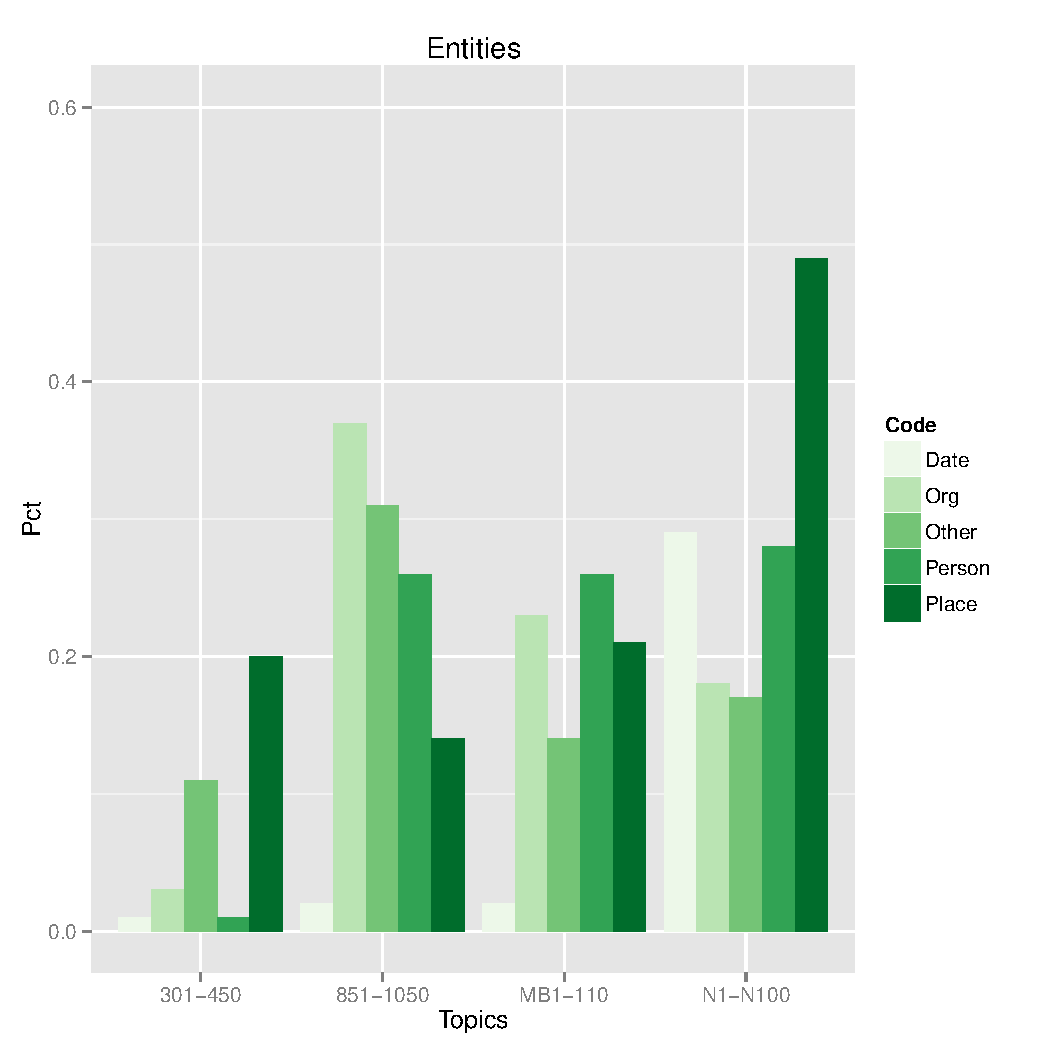
\includegraphics[width=6cm]{plots/topic-groups-ent.pdf}
\end{subfigure}%
\begin{subfigure}{.5\textwidth}
  \centering
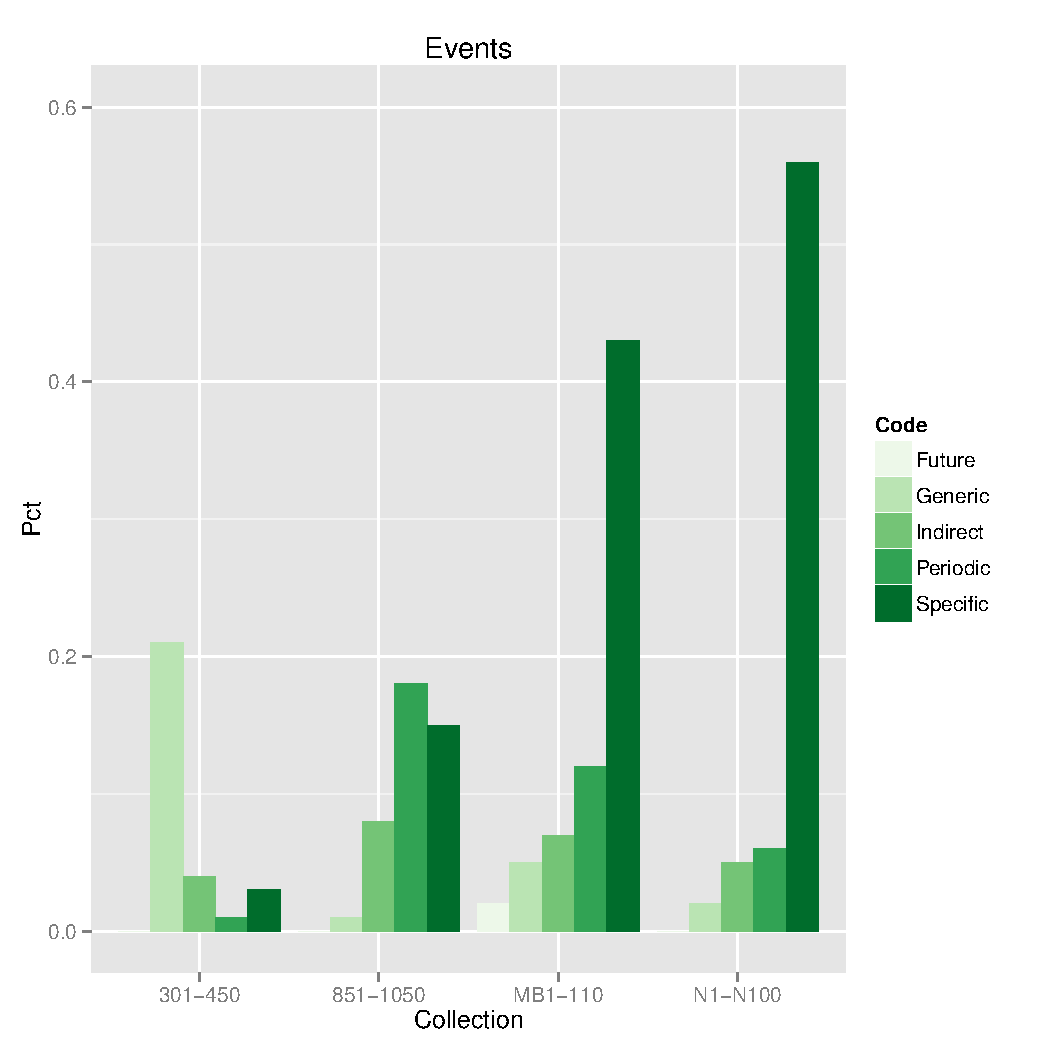
\includegraphics[width=6cm]{plots/topic-groups-evt.pdf}
\end{subfigure}
\caption{Percent of topics in each collection with codes assigned from the (left) entity code group and (right) events code group}
\label{fig.codedist}
\end{figure}


\begin{comment}
\begin{table*}
\small
\begin{tabular}{| l | l | l | l | l | l | l | l | l | l | l |} \hline
Topics & ExpDate &	OrgEnt&	OtherEnt&	PersonEnt&	PlaceEnt&	FutureEvt&	GenericEvt&	IndEvtRef &	PerEvt&	SpecEvt \\ \hline
301-450	&	0.01&	0.03&	0.11&	0.01&	0.20&	0.00&	0.21&	0.04&	0.01&	0.03 \\ \hline
851-1050	&	0.02&	0.37&	0.31&	0.26&	0.14&	0.00&	0.01&	0.08&	0.18&	0.15 \\ \hline
N1-N100	&	0.29&	0.18&	0.17&	0.28&	0.49&	0.00&	0.02&	0.05&	0.06&	0.56 \\ \hline
MB1-110	&	0.02&	0.23&	0.14&	0.26&	0.21&	0.02&	0.05&	0.07&	0.12&	0.43 \\ \hline
\end{tabular}
\caption{Percent of topics with each code assigned by topic group}
\label{table.codedist}
\end{table*}
\end{comment}


\subsection{Reliability}

To assess reliability, a total of 1244 codes were assigned to 330 topics by two coders. The macro percent overlap is 0.71 and  micro percent overlap is 0.83. The per-code overlap is reported in Table \ref{table.overlap}. Higher overlap indicates greater agreement between coders. As expected, some codes have higher agreement than others. Specifically, personal names (0.94), locations (0.91), and explicit dates (0.89) have very high agreement whereas indirect event references (0.19) and generic events (0.45) have lower agreement.

\begin{figure}
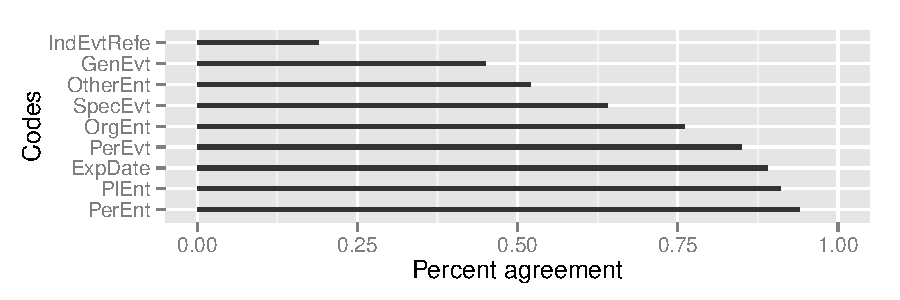
\includegraphics{plots/coder-agreement.pdf}
\end{figure}

\begin{comment}
\begin{table}
\small
\begin{tabular}{| l | l |} \hline
\bf{Code} & \bf{Overlap}  \\ \hline
PersonEntity & 0.94  \\ \hline
PlaceEntity  & 0.91  \\ \hline
ExplicitDate & 0.89   \\ \hline
PeriodicEvent & 0.85   \\ \hline
OrganizationEntity & 0.76  \\ \hline
SpecificEvent & 0.64  \\ \hline
OtherEntity & 0.52  \\ \hline
GenericEvent & 0.45  \\ \hline
IndirectEventReference & 0.19  \\ \hline
\end{tabular}
\caption{Per-code percent overlap }
\label{table.overlap}
\end{table}
\end{comment}

\subsection{Regression analysis}

In this section, were report the results of a logistic regression analysis, predicting the manually assigned categories for each test collection. The resulting models are reported in Table \ref{table.regresults}. 

\begin{table*}
\small
\begin{tabular}{| l | l | l | l | l |} \hline
\bf{Name} & \bf{Model} & \bf{AIC} & \bf{$R^2$} \\ \hline
Novelty 	&  -3.767 + 5.848*SpecEvt + 2.523*OtherEnt & 52 & 0.669 \\ \hline
Novelty (Rel)		&  -3.539 + 7.006*SpecEvt + 2.530*OtherEnt - 7.343*ACF & 49 & 0.706 \\ \hline
Dakka	&  0.134 + 0.878*PlaceEnt  & 205 & 0.020 \\ \hline
Dakka (Rel) 		& -0.917 + 0.393*DPS 	& 155 & 0.263  \\ \hline
Efron	& -1.765 + 2.353*PlaceEnt + 1.410*OtherEnt & 150 & 0.181 \\ \hline
Efron (Rel) 		& -2.727 + 1.965*PlaceEnt + 1.787*OtherEnt  + 0.163*DPS & 118 & 0.377 \\ \hline
Peetz & -0.336 + 1.682*SpecEvt + 0.982*PerEvt + 0.672*PerEnt -0.6175*OrgEnt & 192 & 0.127 \\ \hline
Peetz (Rel) 		& -1.245 + 1.218*SpecEvt + 0.797*PerEvt + 2.835*ACF + 0.002*DPS & 171 & 0.223 \\ \hline
\end{tabular}
\label{table.regresults}
\caption{Logistic regression models for each test collection with and without ACF/DPS variables. Model fit reported based on AIC, cross-validation prediction error, and pseudo-$R^2$.}
\end{table*}

\begin{table*}
\small
\begin{tabular}{| l | l | l | l | l |} \hline
\bf{Collection} 	& \bf{Model} & \bf{AIC} & \bf{$R^2$} \\ \hline
Tweets 2011-12	& 0.722 - 2.332*GenEvt$^\uparrow$  & 141 & 0.043  \\ \hline
Novelty 2003-4 		& -2.658 + 0.920*PlaceEntity$^\uparrow$  + 1.183*SpecificEvent$^\uparrow$  + 2.677*ACF$^\uparrow$  & 130 & 0.10 \\ \hline
AP 			& -0.767 + 0.040*DPS$^\uparrow$  & 204& 0.04 \\ \hline
Blog06		& -1.047 + 0.848*PeriodicEvent + 0.017*DPS$^{\uparrow\uparrow}$ & 195 & 0.065 \\ \hline
LATimes 		& 0.689 + 3.431*ExplicitDate - 0.711*PlaceEntity - 0.116*DPS$^\uparrow$ & 199 &0.054 \\ \hline
\end{tabular}
\label{table.regresults}
\caption{Logistic regression models predicting KL/KDE for each test collection. Model fit reported based on AIC, cross-validation prediction error, and pseudo-$R^2$. $^\uparrow$ indicates p < 0.05. $^{\uparrow\uparrow}$ indicates p < 0.01}
\end{table*}


AP 
	all	0.2166	0.2171	0.0005		0.2183
	t = -5.4211, df = 149, p-value = 1.167e-07	
LATimes
	all	0.1976	0.1984	0.0008		0.2003
	t = -2.0653, df = 149, p-value = 0.02032	
Novelty 03
	all	0.2947	0.2853	-0.0094		0.2986
	t = -3.3995, df = 49, p-value = 0.0006751
Novelty 04
	all	0.3689	0.3643	-0.0046		0.3728
	t = -3.9596, df = 49, p-value = 0.0001213	
Blog06
	all	0.2978	0.2975	-0.0003		0.3013
	t = -3.6519, df = 149, p-value = 0.0001799		
Tweets 2011
	all	0.2251	0.2418	0.0167		0.2448
	t = -4.7387, df = 48, p-value = 9.756e-06	
Tweets 2012
	all	0.1794	0.1907	0.0113		0.1953
	t = -4.9802, df = 58, p-value = 3.018e-06	
	
\subsubsection{Novelty}

We begin with the 2003-2004 Novelty topics. In this case, the response variable is the manually assigned ``opinion'' (0) or ``event'' (1) categories. Following Jones and Dias \cite{Jones2007}, we adopt ``event'' as the temporal category. Logistic regression analysis is performed with and without the ACF and DPS variables. Looking at Table \ref{table.regresults}, SpecificEvent is a useful predictor of the ``event'' category (p < 0.01). This is unsurprising, since the definition of the SpecificEvent code corresponds to the Novelty ``event'' category. Including ACF has a minimal effect. 

\subsubsection{Dakka et al}

Dakka et al provided manual classification of ``time-sensitive queries'' in TREC topics 301-450. As reported in Table \ref{table.regresults}, the DPS variable has a considerable effect in predicting the temporal category. No other variables are significant in this model. This suggests that either 1) Dakka et al relied heavily on the distribution of relevant documents in determining the classification or 2) our model is missing an important explanatory component.

\subsubsection{Efron and Golovchinsky}

Efron and Golovchinsky also classified topics 301-450, in this case identifying only ``recency'' queries. As reported in Table \ref{table.regresults}, both the PlaceEntity and OtherEntity codes are useful predictors of the temporal category. Inclusion of the DPS variable substantially improves model fit. This suggests that the distribution of relevant documents played some role in the determination of topic classes.

\subsubsection{Peetz et al}
Finally, we look at Peetz et al's classification of the Blog06-08 topics 850-1050. In this case, the SpecificEvent and PeriodicEvent code are useful predictors of the temporal category. Including the ACF and DPS variables improves model fit, again suggesting that the distribution of relevant documents played a role in manual classification.

\subsection{Predicting when to use temporal retrieval models}

In the previous section, we report the effectiveness of using the coded topics to predict manually classified temporal categories. In this section, we develop similar to models to predict whether to use a temporal retrieval model for each topic. We use standard query likelihood \cite{XXX} and the kernel density estimate {KDE} temporal model \cite{Efron2014} to determine query temporality. If the average precision (AP) of the KDE model score is greater than the AP of the standard query likelihood score, topics are classified as ``temporal.''  If the QL model is more effective, the topic is classified as ``non-temporal.'' As in the previous section

Instead of testing these retrieval models in conventional evaluation, we instead use the resulting classification for comparison to the manual classifications and the results of the above described content analysis.

The content analysis relies on a manual review and interpretation of the topic text with some investigation of related contexts. The original manual classifications relied on a combination of manual interpretation of topic text and interpretation or heuristic classification based on the distribution of true-relevant documents. The retrieval models rely on the distribution of pseudo-relevant documents. As a final measure, we adopt the cross-correlation function (CCF) used by Amodeo et al \cite{Amodeo2011} to measure the correlation of the true-relevant and pseudo-relevant document distributions. 

The final analysis will include a regression analysis of the above features including the qualitative codes, previously assigned classifications, automatic classification based on retrieval performance and the CCF.


\section{Conclusions}


%ACKNOWLEDGMENTS are optional
\section{Acknowledgments}
This section is optional

%
% The following two commands are all you need in the
% initial runs of your .tex file to
% produce the bibliography for the citations in your paper.


\bibliographystyle{abbrv}
\bibliography{temporalir}  

\section*{Appendix: Codebook}
\begin{table*}[H]
\resizebox{\textwidth}{!}{%
\begin{tabular}{| p{3cm} | p{6cm}  | p{6cm} |} \hline
\bf{Code} & \bf{Description} & \bf{Examples}  \\ \hline
Specific Event & Something significant that happens at a specific time and place. Code title and description in concert, even if title does not contain event specifics. & Mount Pinatubo erruption on June 15, 1991; 2008 State of the Union; Hurricane Hugo \\ \hline
Generic Event & Use this code when the topic refers to more than one specific event or a class or type of event. Only use this code if every instance of the event type would be newsworthy (i.e., a specific event) and the central topic of a news article. & Earthquakes, volcano erruptions, elections, disputes, strikes \\ \hline
Indirect Event Reference & Apply this code to indicate when the topic might be indirectly referring to a *specific* event. Use only if you need to turn to external information to identify potential specific events (e.g., your personal knowledge, wikipedia). Do not use if specific event information is contained in the description. & Legally assisted suicide, related to Kevorkian controversy. Partial birth abortion ban, related to partial birth abortion ban legislation. Surrogacy related to Baby M. \\ \hline
Periodic Event & Apply this code to indicate when an event is periodic, recurring at regular, predictable intervals. Never double-code as SpecificEvent or as an entity even though periodic events are often named entities. & Super bowl, Nobel awards, Oscars, State of the Union \\ \hline
FutureEvent & Apply this code to indicate when a topic refers to a future predicted specific event. Never double-code as SpecificEvent. & 2020 Fifa, 2016 Summer Olympics \\ \hline
Person Entity & Apply this code to identify personal names in topics. & President Bush; Sasha Cohen;  \\ \hline
Place Entity & Apply this code to identify places in topics. Limit to proper names. Also apply to references to nations, governments or government bodies. & Peru; Africa; African; European; Atlanta \\ \hline
Organization Entity & Apply this code to identify organizations in topics. Limit to proper names. Do not apply to references to governments (e.g., United States), use PlaceEntity instead. & Hitachi Data Systems; U.S. Congress; \\ \hline
Other Entity & Apply this code to named entities that are not people, places or organizations. Limit to proper names. Includes movies, books., etc. & Hubble Telescope; The Avengers; Euro	\\ \hline
Explicit Date & Apply this code to identify explicit dates. & 1988; June 15, 1991; October 2007; Monday \\ \hline
\end{tabular}}
\caption{Codebook}
\label{table.codebook}
\end{table*}






\end{document}
